\section{Web Data Inspector}
\label{sec:web-data-inspector}

Web Data is a collection of heterogeneous datasets, coming from a variety of sources and spanning over many diverse domains. Some datasets are created by integrating others. Datasets owners  expose links between other datasets and their own in order to improve their connectivity to the rest of Web Data. This thoughtful process, which is not an objective per se, allows more relevant information to be accessible for the user. As a user trying to retrieve some information from this heterogeneous collection of datasets, it is necessary to have sufficient insight into the dataset of interest in order to formulate queries: the user needs to understand how the data is structured, how a dataset is connected to others, and to assess in some way the quality of the data.

In this section, we present the \emph{Web Data Inspector} as a tool for inspecting the edges of a dataset through the use of graph summaries.

\subsection{Views into a Dataset}

Based on the graph summary, the Web Data Inspector presents different views of a dataset. This tool was part of the Sindice~\cite{oren:2008:sdl} project; its home page, not anymore accessible with the end of the Sindice\footnote{\url{http://www.dataversity.net/end-support-sindice-com-search-engine-history-lessons-learned-legacy-guest-post/}} project, is shown in Figure~\ref{fig:wdi:home-page} and provides the user with a text box where he can enter the dataset's name of interest --- here, the domain name of the web site. By clicking the ``Check'' button, the user will be provided with several views useful in exploring the content and the structure of the chosen dataset.

Also, from the home page, the user has the possibility to choose an RDF class or an RDF property and then, upon clicking the ``Check'' button, the user is shown the provenance datasets of such RDF element (classes or properties) as well as its relationships with other RDF elements. In order to provide such information, a summary of the dataset collection is generated and is presented thanks to the RDF data model described in Section~\ref{chap03:sec:wd-mgnt}.

\begin{figure}
	\centering
	\resizebox{.9\textwidth}{!}{
		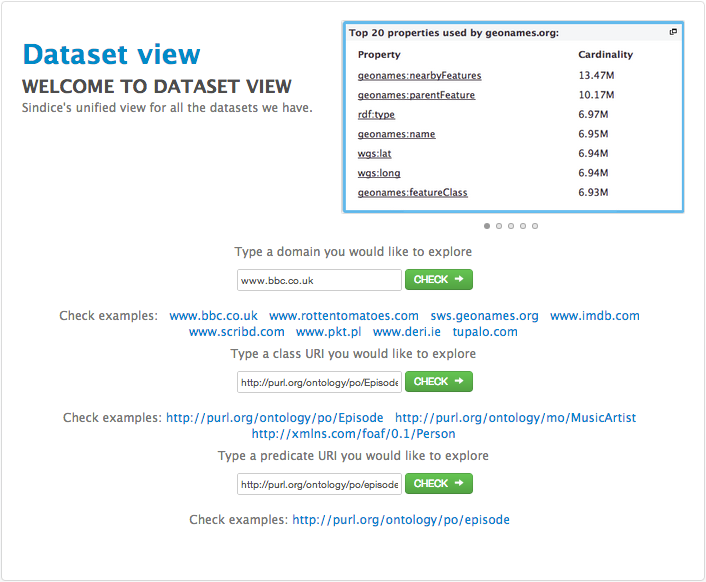
\includegraphics[scale=1]{exploiting/wlv/images/home-page}
	}
	\caption{Web Data Inspector - home page}
	\label{fig:wdi:home-page}
\end{figure}

In the next subsections, we describe in more detail the different views that the user is provided with when exploring a dataset using the Web Data Inspector. 

\subsubsection{General View}

The general view tab as depicted in Figure~\ref{fig:wdi:generalView} shows a summary of some of the particular dataset's properties and statistics. This includes the domain address of the dataset and the size in terms of triples and documents. Further details and analysis is found in the other tabbed sections: ``Inside this dataset'', ``To/from datasets'', and ``Third party''.

\begin{figure}
	\centering
	\resizebox{.9\textwidth}{!}{
		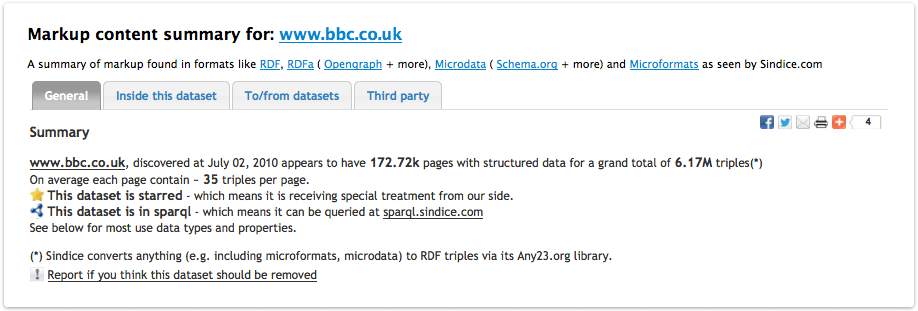
\includegraphics[scale=1]{exploiting/wlv/images/general.png}
	}
	\caption{Web Data Inspector - general view}
	\label{fig:wdi:generalView}
\end{figure}

\subsubsection{Inside This Dataset}

The ``Inside this dataset'' tab as depicted in Figure~\ref{fig:wdi:insideThisDataset} delves deeper into the dataset to explore and present information about the RDF properties and classes used within. This view shows the links that are classified as internal only to the dataset. From this view, a user may learn more about the structure and content of the dataset.

The first two boxes present to the user the top properties and classes used in the dataset.
The next two present to the user a property, and when selecting a specific one, the classes that are connected by that property.
The last two boxes report the opposite: when selecting a specific pair of classes, the properties connecting the two are presented.

We present below a SPARQL query that is used for retrieving the top properties and classes occurring in a dataset. The query is executed over the graph summary of the inspected data collection. The dataset that is being inspected is denoted as ``MYGRAPH'' in the following query. The output of this query is used for populating the first two boxes on the top in Figure~\ref{fig:wdi:insideThisDataset}.

\begin{minted}[linenos,frame=lines,framesep=1mm]{sparql}
SELECT ?type ?label (SUM(?nb) AS ?total) WHERE {
  {
    BIND ("class" AS ?type)
    ?n a :SNode;
       :origin <MYGRAPH>;
       :statistic ?nb;
       :feature / :label ?label .
  } UNION {
    BIND ("property" AS ?type)
    ?e a :SEdge;
       :origin <MYGRAPH>;
       :statistic ?nb;
       :label ?label .
  }
}
GROUP BY ?type ?label
\end{minted}

In the following SPARQL query, we describe how the statistics for the last four boxes of Figure~\ref{fig:wdi:insideThisDataset} are retrieved from the graph summary. The query returns
\begin{inparaenum}[(a)]
\item the class of the subject component;
\item the class of the object component; and
\item the total number of links that connects the previous two classes for a specific property.
\end{inparaenum}

\begin{minted}[linenos,frame=lines,framesep=1mm]{sparql}
SELECT ?sourceClass ?targetClass ?property (SUM(?nb) AS ?total) WHERE {
  ?source a :SNode; :origin <MYGRAPH>; :feature / :label ?sourceClass .
  ?target a :SNode; :origin <MYGRAPH>; :feature / :label ?targetClass .
  ?e a :SEdge;
     :origin <MYGRAPH>;
     :source ?source;
     :target ?target;
     :statistic ?nb;
     :label ?property .
}
GROUP BY ?sourceClass ?property ?targetClass
\end{minted}

\begin{figure}
	\centering
	\resizebox{\textwidth}{!}{
		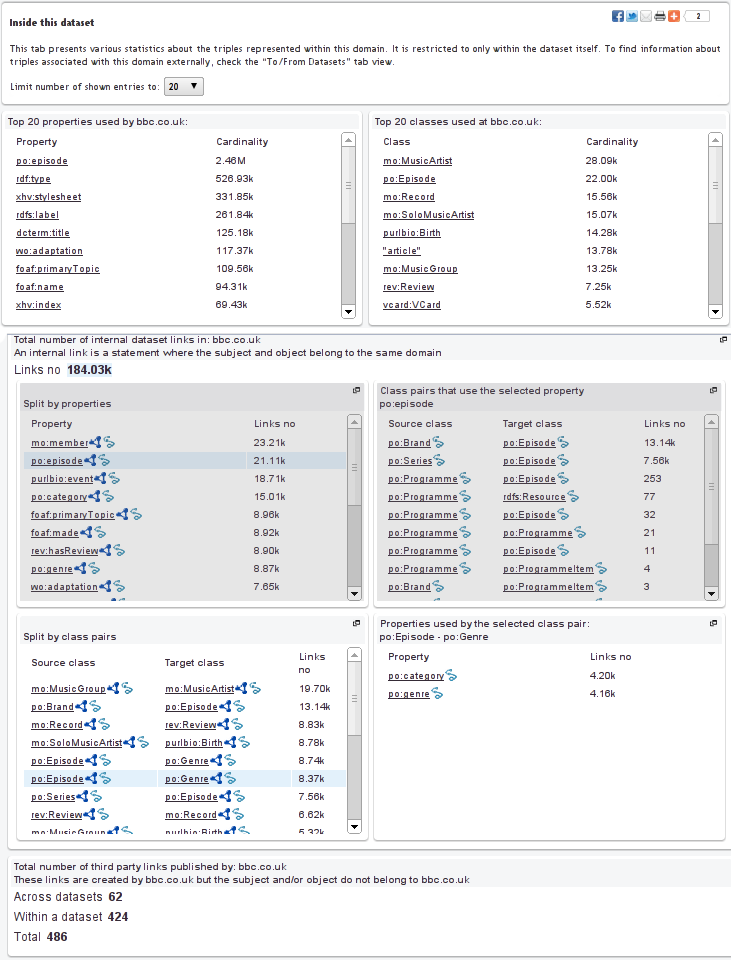
\includegraphics[scale=1]{exploiting/wlv/images/insideThisDataset.png}
	}
	\caption{Web Data Inspector - inside this dataset}
	\label{fig:wdi:insideThisDataset}
\end{figure}

\subsubsection{To/From This Dataset}

The ``To/from datasets'' tab as depicted in Figure~\ref{fig:wdi:toFromThisDataset} presents the existing relationships this dataset has with other datasets. From here, exploration can span across the many domains that the particular dataset is linked with.

The first two boxes present the datasets the current dataset being inspected connects to. Instead, the next two boxes report on the datasets that link to the current dataset.

We show below a SPARQL query that is used for retrieving the data necessary for the boxes depicted in Figure~\ref{fig:wdi:toFromThisDataset}. We denote with ``MYGRAPH'' the dataset being explored, e.g., \emph{bbc.co.uk} in the figure. The query retrieves links that connects to and from the ``MYGRAPH'' dataset; ``\emph{to}'' the dataset is shown in the first block of the UNION, while ``\emph{from}'' the dataset is shown in the second block.

\begin{minted}[linenos,frame=lines,framesep=1mm]{sparql}
SELECT ?sourceDomain ?targetDomain ?property (SUM(?nb) AS ?total) WHERE {
  ?e a :SEdge;
     :origin <MYGRAPH>;
     :label ?property;
     :statistics ?nb .
  {
    BIND (<MYGRAPH> AS ?sourceDomain)
    ?e :source [ :origin <MYGRAPH> ];
       :target [ :origin ?targetDomain ] .
  } UNION {
    BIND (<MYGRAPH> AS ?targetDomain)
    ?e :source [ :origin ?sourceDomain ];
       :target [ :origin <MYGRAPH> ] .
  }
}
GROUP BY ?sourceDomain ?targetDomain ?property
\end{minted}

\begin{figure}
	\centering
	\resizebox{\textwidth}{!}{
		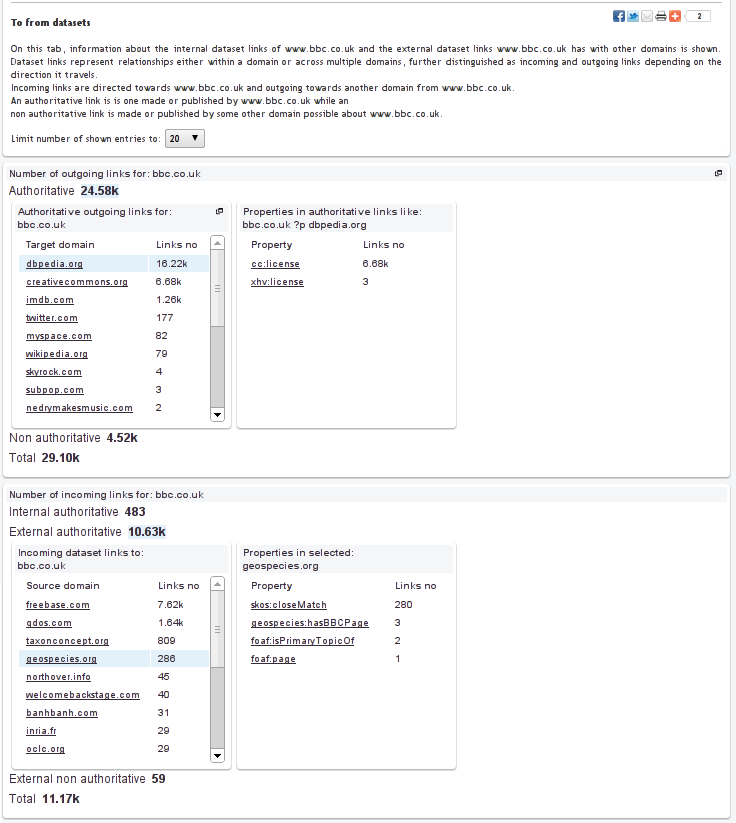
\includegraphics[scale=1]{exploiting/wlv/images/toFromDataset}
	}
	\caption{Web Data Inspector - to/from this dataset}
	\label{fig:wdi:toFromThisDataset}
\end{figure}

\subsubsection{Third-Party Links}

The edge authority as defined in Definition~(\ref{def:edge-authority}) helps dataset owners to distinguish another important aspect: third-party links. These represent links that do not have authority; the ability to differentiate a link as being a \emph{third-party link} helps to discover if the link is incorrect or specify relationship that the owner does not explicitly agree with. In some cases, these links can be connotative to the idea of e-mail spam.

The ``Third-party links'' tab as depicted in Figure~\ref{fig:wdi:thirdPartyLinks} shows to the user information about third-party links, inferred from the graph summary.
Statistics reported in this section differ from those reported in the ``To/From This Dataset'' by filtering links which were not published in the inspected dataset, e.g., \emph{bbc.co.uk} in the figure.

\begin{minted}[linenos,frame=lines,framesep=1mm]{sparql}
SELECT ?PublishedOn ?sourceDomain ?targetDomain
       ?property (SUM(?nb) AS ?total) WHERE {
  ?e a :SEdge;
     :origin ?PublishedOn;
     :label ?property;
     :statistics ?nb .
  {
    BIND (<MYGRAPH> AS ?sourceDomain)
    ?e :source [ :origin <MYGRAPH> ];
       :target [ :origin ?targetDomain ] .
  } UNION {
    BIND (<MYGRAPH> AS ?targetDomain)
    ?e :source [ :origin ?sourceDomain ];
       :target [ :origin <MYGRAPH> ] .
  }
  FILTER ?PublishedOn != <MYGRAPH>
}
GROUP BY ?PublishedOn ?sourceDomain ?targetDomain ?property
\end{minted}

\begin{figure}
	\centering
	\resizebox{.9\textwidth}{!}{
		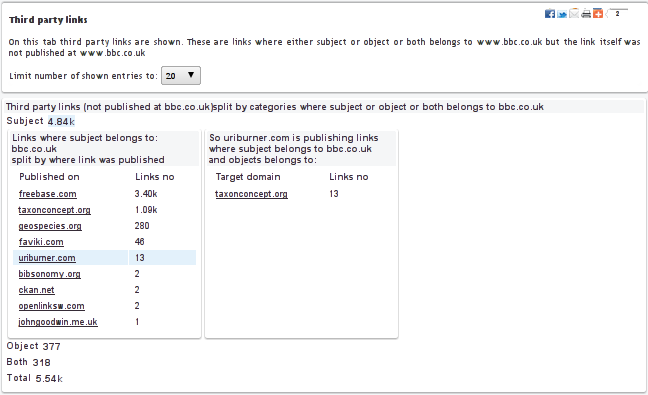
\includegraphics[scale=1]{exploiting/wlv/images/thirdPartyLinks}
	}
	\caption{Web Data Inspector - third party links view}
	\label{fig:wdi:thirdPartyLinks}
\end{figure}

\subsection{Evaluation}

In this section, we show how the Web Data Inspector tool works across some notable datasets: \textbf{bbc.co.uk}, \textbf{sws.gonames.org}, and \textbf{www.rottentomatoes.com}.
Statistics reported in this evaluation date from April 2012.

\subsubsection{bbc.co.uk}

The dataset ``bbc.co.uk'' uses RDFa to annotate their ``Programmes'' and ``Music'' websites. As depicted in Figure~\ref{fig:wdi:generalView}, there are over 6M triples that cover brands, series (seasons), episodes, artists, broadcast events, broadcast services, etc. The top three most used classes in the ``bbc.co.uk'' dataset are: ``article'' which appears 44.12K times, ``mo:MusicArtist'' 24.18K times and ``vcard:Name'' 20.48K times. The top three most popular properties are ``po:episode'' with 2.67M occurrences, ``rdfs:label'' with 216.78K and ``wo:adaptation'' with 139.14K, as depicted in Figure~\ref{fig:wdi:insideThisDataset}.

The ``bbc.co.uk'' dataset includes links to further URIs, allowing the user to discover more data, e.g. about members of a band or about a certain series episode. It also includes a ``owl:sameAs'' link with 21.61K occurrences to the corresponding DBpedia resource, allowing the user to aggregate more data about that band, extracted from Wikipedia's infoboxes. From the ``To/from dataset'' view, a user may note that there are about 3K links that link ``bbc.co.uk'' to well known datasets such as ``dbpedia.org'', ``myspace.com'', and ``imdb.com'' as reported by the ``outgoing links'' box. On the incoming links side, the user can observe that few datasets are linked to ``bbc.co.uk'' as there are only 275 links that link other datasets like ``freebase.com'' and ``dbpedia.org'' to ``bbc.co.uk''.

\subsubsection{sws.geonames.org}

The dataset ``sws.geonames.org'' is a dump dataset rather than a website which provides over 129M triples, as depicted in Figure~\ref{fig:wdi:generalView}, about countries and geographical locations. The user can see what classes occur in that dataset such as ``geonames:Feature'' which appears 7.85M times, ``wgs:Point'' 4.36K times and ``foaf:Agent'' with 2.41K occurrences and properties such as ``geonames:nearbyFeatures'' with 14.28M occurrences, ``geonames:name'' with 7.89M occurrences and ``geonames:parentFeature'' with 7.88M occurrences.

The ``sws.geonames.org'' dataset includes over 4M links to resources from other datasets like ``identi.ca'', ``nytimes.com'', or ``dbpedia.org'' as depicted by the outgoing links box in Figure~\ref{fig:wdi:toFromThisDataset}. This dataset is also well linked to by other datasets like ``naplesplus.us'', ``dbpedia.org'' or ``geospecies.org'' with over 274K incoming links.

\subsubsection{www.rottentomatoes.com}

Rotten Tomatoes is a film review aggregator which provides reviews, information, and news of films. It contains over 11M triples, as depicted in Figure~\ref{fig:wdi:generalView}, and it uses several proprietary vocabularies. Among the most popular classes, a user may note the classes ``actor'' which appears 147.19K times, ``sorg:Person'' 31.00K times, ``sorg:AggregateRating'' 2.94K times and ``video.movie'' 2.77K times.

The linkage for this dataset with others is very poor as reported to the user by the number 0 for the outgoing/incoming links box in Figure~\ref{fig:wdi:toFromThisDataset}. A possible improvement of the dataset might be to increase the linkage of the dataset with links to well known datasets like ``dbpedia.org'' or specific datasets like ``imdb.com''.

\subsection{Dataset Improvements thanks to Web Data Inspector}

In this section we show how the results of the Web Data Inspector can be used as suggestions for improving one's dataset. Being able to see the classes and the properties of his dataset, the dataset owner is able to have a deep understanding of his dataset. The user can determine if the dataset graph is shaped as planned.

For example, a user may assume that his dataset contains the ``foaf:Person'' class which has, among others, the ``foaf:name'' and ``foaf:homepage'' properties. From the number of the occurrences of these properties, a dataset owner can decide if his dataset is as intended: if it is expected that most people mentioned in the dataset have an homepage, then this should be reflected in similar numbers for the occurrences of the ``foaf:name'' and ``foaf:homepage'' properties.

Also, a dataset owner can identify possible mistakes such as typos in the classes/properties names. For example, it is well known that ``foaf:name'' is a property of the FOAF vocabulary but that ``foaf:naem'' is not.
